\graphicspath{{Figs/scattering/}}

\chapter{Scattering: The DOIT solver}
 \label{sec:doit}

\starthistory
 020601 & Created and written by Claudia Emde\\ 
 050223 & Rewritten by Claudia Emde, mostly taken from Chapter 4 of Claudia Emde's PhD thesis \\
 091014 & Moved from user guide to theory document.\\
\stophistory

The \textindex{Discrete Ordinate ITerative (DOIT) method} is one of the
scattering algorithms in ARTS. The DOIT method is unique because a discrete
ordinate iterative method is used to solve the scattering problem in a
spherical atmosphere. Although the DOIT module is implemented for 1D and 3D
atmospheres, it is strongly recommended to use it only for 1D, because the
Monte Carlo module (Chapter \ref{sec:montecarlo}) is much more
appropriate for 3D calulations. More appropriate in the sense that it is much
more efficient. A literature review about scattering models for the microwave
region, which is presented in \citet{sreerekha04:_devel_rt_ghz_wp1}, shows that
former implementations of discrete ordinate schemes are only applicable for
(1D-)plane-parallel or 3D-cartesian atmospheres. All of these algorithms can
not be used for the simulation of limb radiances. A description of the DOIT
method, similar to what is presented in this chapter, has been published in
\citet{emde04:_doit_jgr} and in \citet{emde05:_phdthesis}.


\section{Radiation field}
\label{sec:doit:rad_field}
The Stokes vector depends on the
position in the cloud box and on the propagation direction specified
by the zenith angle ($\ZntAng$) and the azimuth angle ($\AzmAng$). All
these dimensions are discretized inside the model; five
numerical grids are required to represent the \textindex{radiation field}
$\IFld$:
\begin{eqnarray}
  \vec{\Prs} &= \{ \Prs_1, \Prs_2, ... , \Prs_{N_\Prs}\}, \nonumber \\
  \vec{\Lat} &= \{ \Lat_1, \Lat_2, ... , \Lat_{N_\Lat}\}, \nonumber \\
  \vec{\Lon} &= \{\Lon_1, \Lon_2, ... , \Lon_{N_\Lon}\}, \\
  \vec{\ZntAng} &= \{\ZntAng_1, \ZntAng_2, ... , \ZntAng_{N_\ZntAng}\}, \nonumber \\
  \vec{\AzmAng} &= \{\AzmAng_1, \AzmAng_2, ... , \AzmAng_{N_\AzmAng}\}. \nonumber 
\end{eqnarray}
Here $\vec{\Prs}$ is the pressure grid, $\vec{\Lat}$ is the latitude
grid and $\vec{\Lon}$ is the longitude grid.
The radiation field is a set of Stokes vectors ($N_\Prs\times N_\Lat
\times N_\Lon \times N_\ZntAng \times N_\AzmAng$ elements) for all
combinations of positions and directions:
\begin{eqnarray}
  \IFld &= \{ \StoVec_1(\Prs_1,\Lat_1, \Lon_1, \ZntAng_1, \AzmAng_1),
  \StoVec_2(\Prs_2,\Lat_1, \Lon_1, \ZntAng_1, \AzmAng_1), ... , \nonumber \\ 
  &\StoVec_{N_\Prs\times N_\Lat \times N_\Lon \times N_\ZntAng \times N_\AzmAng}
  (\Prs_{N_\Prs},\Lat_{N_\Lat}, \Lon_{N_\Lon}, \ZntAng_{N_\ZntAng}, 
  \AzmAng_{N_\AzmAng}) \}. 
\end{eqnarray}
In the following we will use the notation
\begin{eqnarray}
  & i = 1 \ldots N_\Prs  \nonumber \\
  & j = 1 \ldots N_\Lat  \nonumber \\
  \IFld = \left\{\StoVec_{ijklm}\right\}  \hspace{5ex}&
  k = 1 \ldots N_\Lon. \\
  &  l = 1 \ldots N_\ZntAng  \nonumber \\
  &  m = 1 \ldots N_\AzmAng  \nonumber
\end{eqnarray}

\section{Vector radiative transfer equation solution} 
\label{sec:doit:VRTE_sol}

Figure \ref{fig:scattering:iteration_scheme} shows a schematic of the iterative
method, which is applied to solve the \textindex{vector radiative transfer
equation} (compare Equation \ref{eq:rtetheory:VRTE})
\begin{eqnarray}
  \frac {\DiffD\StoVec(\PDir, \nu, T)}{\DiffD s} =
    &{}-\EnsAvr{\ExtMat(\PDir, \nu, T)} \StoVec(\PDir, \nu, T) +
    \EnsAvr{\AbsVec(\PDir, \nu, T)} \rlap{$B(\nu, T)$} \\
    &{}+ \int_{4\pi} \DiffD\PDir' \EnsAvr{\PhaMat(\PDir, \PDir', \nu, T)} \StoVec(\PDir', \nu, T),
\end{eqnarray}
where $\StoVec$ is the specific intensity vector, $\EnsAvr\ExtMat$
is the ensemble-averaged extinction matrix, $\EnsAvr\AbsVec$ is the
ensemble-averaged absorption vector, $B$ is the 
Planck function and $\EnsAvr\PhaMat$ is the ensemble-averaged
phase matrix.  Furthermore $\nu$ is the frequency of the radiation,
$T$ is the temperature, $\DiffD s$ is a path-length-element of the
propagation path and $\PDir$ the propagation direction.
The vector radiative transfer equation is explained in more detail in
Section \ref{sec:rtetheory:theory_rte}. 


\begin{figure}[t!]
  \fbox{
  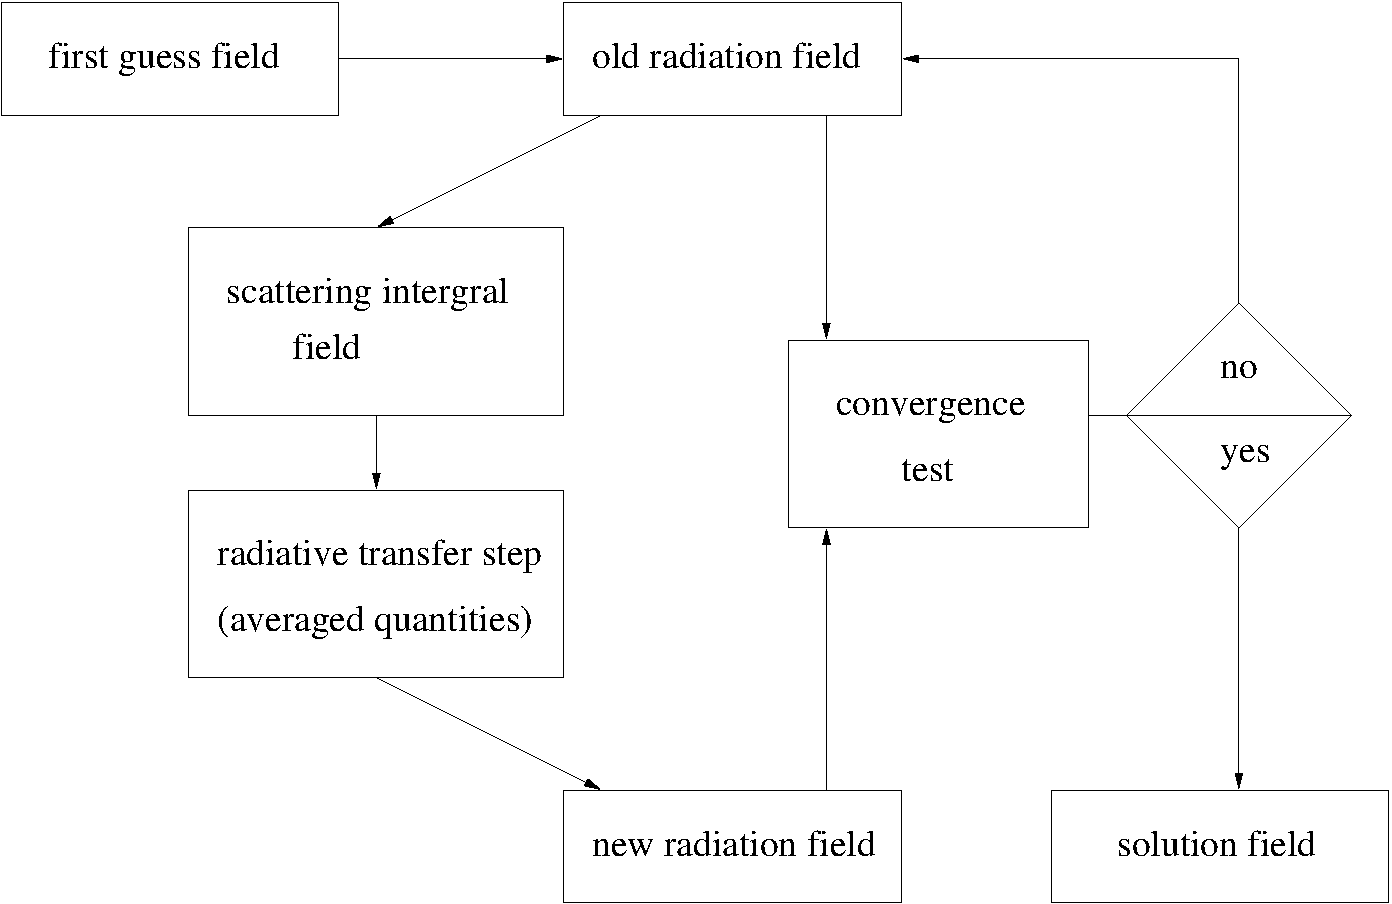
\includegraphics[width=.95\hsize]{iteration_scheme}}
  \caption{Schematic of the iterative method to solve the VRTE in the cloud box.}
  \label{fig:scattering:iteration_scheme}
\end{figure}

The \emph{first guess field}
\begin{equation}
  \IFld^{(0)} = \left\{\StoVec^{(0)}_{ijklm}\right\},
\end{equation}
is partly determined by the boundary condition given by the radiation
coming from the clear sky part of the atmosphere traveling into the
cloud box.  Inside the cloud box an arbitrary field can be chosen as a
first guess. In order to minimize the number of iterations it should
be as close as possible to the solution field.

The next step is to solve the scattering integrals
\begin{equation}
  \EnsAvr{\AmpMat^{(0)}_{ijklm}} = \int_{4\pi} \DiffD \PDir'
  \EnsAvr{\PhaMat_{ijklm}} \StoVec_{ijklm}^{(0)},
  \label{eq:scattering:scat-int}
\end{equation}
using the first guess field, which is now stored in a variable
reserved for the \emph{old radiation field}. For the integration we
use equidistant angular grids in order to save computation time (cf.
Section \ref{sec:doit:grid_opt_interp}).  The radiation field, which is
generally defined on finer angular grids ($\vec{\AzmAng},
\vec{\ZntAng}$), is interpolated on the equidistant angular grids.
The integration is performed over all incident directions $\PDir'$ for
each propagation direction $\PDir$.  The evaluation of the scattering
integral is done for all grid points inside the cloud box. The
obtained integrals are interpolated on $\vec{\AzmAng}$ and
$\vec{\ZntAng}$.  The result is the first guess \emph{scattering
  integral field} ${\mathcal S}^{0}$:
\begin{equation}
  \SFld^{(0)} = \left\{\EnsAvr{\SVec^{(0)}_{ijklm} }\right\}.  
\end{equation}

Figure \ref{fig:scattering:average} shows a propagation path step from a grid
point $\VctStl{P} = (\Prs_i, \Lat_j, \Lon_k)$ into direction $\PDir =
(\ZntAng_l, \AzmAng_m)$. The radiation arriving at $\VctStl{P}$ from the
direction $\PDir'$ is obtained by solving the linear
differential equation:
\begin{equation}
  \frac{\DiffD \StoVec^{(1)}}{\DiffD s} =
  -\overline{\EnsAvr\ExtMat}  \StoVec^{(1)} + \overline{\EnsAvr\AbsVec}\,  \bar{B}
  +\overline{\EnsAvr{\SVec^{(0)}}},
  \label{eq:scattering:vrte-fs-av}
\end{equation}
where $\overline{\EnsAvr\ExtMat}$, $\overline{\EnsAvr\AbsVec}$, $\bar{B}$ and $\overline{\EnsAvr{\SVec^{(0)}}} $ are \emph{averaged quantities}.  This equation
can be solved analytically for constant coefficients. Multi-linear
interpolation gives the quantities $\ExtMat', \AbsVec',
\SVec'$ and $T'$ at the intersection point $\VctStl{P}'$.  To calculate the radiative transfer from $\VctStl{P}'$ towards $\VctStl{P}$ all quantities are approximated by
taking the averages between the values at $\VctStl{P}'$ and $\VctStl{P}$. The average value of the temperature is used to get the
averaged Planck function $\bar{B}$.

\begin{figure}[t!]
  \centering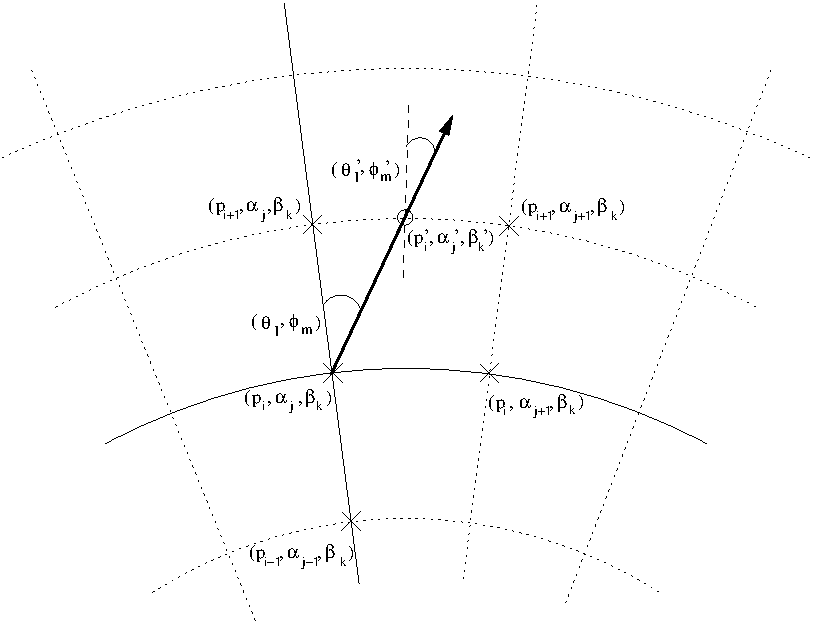
\includegraphics[width=.8\hsize]{average}
  \caption{Path from a grid point ($(\Prs_i, \Lat_j, \Lon_k)$~-~($\times$)) to the intersection point ($(\Prs_i', \Lat_j', \Lon_k')$~-~($\circ$)) with the next grid cell boundary. Viewing direction is specified by $(\ZntAng_l, \AzmAng_m)$ at ($\times$) or $(\ZntAng_l', \AzmAng_m')$ at ($\circ$).}
  \label{fig:scattering:average}
\end{figure}

The solution of Equation \ref{eq:scattering:vrte-fs-av} is found analytically using
a matrix exponential approach: % \FIXME  (see \appref{app:A}):
\begin{equation}
  \StoVec^{(1)} =
  e^{-\overline{\EnsAvr\ExtMat}  s} \StoVec^{(0)} + 
  \left( \IdnMtr -  e^{-\overline{\EnsAvr\ExtMat} s} \right)
  \overline{\EnsAvr\ExtMat}^{\,-1} \left(\overline{\EnsAvr\AbsVec}\,
    \bar{B} + \overline{\EnsAvr{\SVec^{(0)}}} \right),
  \label{eq:scattering:VRTE_sol}
\end{equation}
where \IdnMtr\ denotes the identity matrix and $\StoVec^{(0)}$ the
initial Stokes vector.  The \emph{radiative transfer step} from $\VctStl{P}'$ to $\VctStl{P}$ is calculated, therefore $\StoVec^{(0)}$ is
the incoming radiation at $\VctStl{P}'$ into direction
$(\ZntAng_l', \AzmAng_m')$, which is the first guess field
interpolated on $\VctStl{P}'$.  This radiative transfer step
calculation is done for all points inside the cloud box in all
directions. The resulting set of Stokes vectors ($\StoVec^{(1)}$ for
all points in all directions) is the first order iteration field
$\IFld^{(1)}$:
\begin{equation}
  \IFld^{(1)} = \left\{ \StoVec^{(1)}_{ijklm}\right\}.  
\end{equation}
The first order iteration field is stored in a variable reserved for the 
\emph{new radiation field}. 

In the \emph{convergence test} the \emph{new radiation field} is
compared to the \emph{old radiation field}. For the difference field,
the absolute values of all Stokes vector elements for all cloud box
positions are calculated. If one of the differences is larger than a
requested accuracy limit, the convergence test is not fulfilled. The
user can define different convergence limits for the different Stokes
components.

If the convergence test is not fulfilled, the first order iteration
field is copied to the variable holding the \emph{old radiation field}, 
and is then used to evaluate again the scattering integral at all
cloud box points:
\begin{equation}
  \EnsAvr{\SVec^{(1)}_{ijklm}} = \int_{4\pi} \DiffD \PDir'
  \EnsAvr\PhaMat \StoVec^{(1)}_{ijklm}.
\end{equation}
The second order iteration field
\begin{equation}
  \IFld^{(2)} = \left\{\StoVec^{(2)}_{ijklm}\right\},  
\end{equation}
is obtained by solving
\begin{equation}
  \frac{\DiffD \StoVec^{(2)}}{\DiffD s} =
  -\overline{\EnsAvr\ExtMat}  \StoVec^{(2)} + \overline{\EnsAvr\AbsVec}\,  \bar{B}
  +\overline{\EnsAvr{\SVec^{(1)}}},
\end{equation}
for all cloud box points in all directions.  This equation contains
already the averaged values and is valid for specified positions and
directions.

As long as the convergence test is not fulfilled the scattering integral fields and higher order iteration
fields are calculated alternately. 

We can formulate a differential equation for the $n$-th order
iteration field. The scattering integrals are given by
\begin{equation}
 \EnsAvr{\SVec^{(n-1)}_{ijklm}} = \int_{4\pi} \DiffD \PDir'
  \EnsAvr\PhaMat \StoVec^{(n-1)}_{ijklm},
\end{equation}
and the differential equation for a specified grid point into a
specified direction is
\begin{equation}
  \frac{\DiffD \StoVec^{(n)}}{\DiffD s} =
  -\overline{\EnsAvr\ExtMat}  \StoVec^{(n)} + \overline{\EnsAvr\AbsVec} \,\bar{B}
  +\overline{\EnsAvr{\SVec^{(n-1)}}}.
\end{equation}
Thus the \emph{$n$-th order iteration field }
\begin{equation}
  \IFld^{(n)} = \left\{ \StoVec^{(n)}_{ijklm} \right\},  
\end{equation}
is given by
\begin{equation}
  \StoVec^{(n)} =  e^{-\overline{\EnsAvr\ExtMat}
    s} + \cdot\StoVec^{(n-1)}  (\IdnMtr - e^{-\overline {\EnsAvr\ExtMat
    s}} ) \overline{\EnsAvr\ExtMat} ^{\,-1} ( \overline{\EnsAvr\AbsVec}\,\bar{B} + \overline{\EnsAvr{\SVec^{(n-1)}}} ),
\end{equation}
for all cloud box points and all directions defined in the numerical
grids.

If the convergence test
\begin{equation}
  \Abs{\StoVec^{(N)}_{ijklm} \left( \Prs_i, \Lat_j, \Lon_k, \ZntAng_l, \AzmAng_m\right)  -  \StoVec^{(N-1)}_{ijklm} \left( \Prs_i, \Lat_j, \Lon_k, \ZntAng_l, \AzmAng_m\right)} < \VctStl{\epsilon},
  \label{eq:scattering:conv_test}
\end{equation}
is fulfilled,
 a solution to the vector radiative transfer equation 
has been found:
\begin{equation}
  \IFld^{(N)} = \left\{ \StoVec^{(N)}_{ijklm} \right\}. 
\end{equation}



\section{Scalar radiative transfer equation solution}
\label{sec:doit:scattering:solution_rte_scalar}

In analogy to the \emph{scattering integral} vector field the scalar
scattering integral field is obtained:
\begin{equation}
  \EnsAvr{S^{(0)}_{ijklm}}  = \int_{4\pi} \DiffD \PDir' \EnsAvr{ Z_{11}} I^{(0)}_{ijklm}.
\end{equation}
The \emph{\textindex{scalar radiative transfer}} equation (compare
Equation~\ref{eq:rtetheory:SRTE}) with a
fixed scattering integral is
\begin{equation}
  \label{eq:scattering:SRTE-Int}
  \frac{\DiffD I^{(1)}}{\DiffD s} = -\EnsAvr{ K_{11}} I^{(1)}
  + \EnsAvr{a_1} B +\EnsAvr{S^{(0)}}.
\end{equation}
Assuming constant coefficients this equation is solved analytically
after averaging extinction coefficients, absorption coefficients,
scattering vectors and the temperature. The averaging procedure is done
analogously to the procedure described for solving the VRTE.  The
solution of the averaged differential equation is
\begin{equation}
\label{eq:scattering:SRTE_sol}
  I^{(1)} = I^{(0)} e^{-\overline{\EnsAvr{K_{11}}} s} +
  \frac{\overline{\EnsAvr{a_1}}\, 
    \bar{B} + \overline{\EnsAvr{ S^{(0)}}} }
  {\overline{\EnsAvr{ K_{11}}} }
  \left(1-e^{-\overline{\EnsAvr{K_{11}}} s}\right),
\end{equation}
where $I^{(0)}$ is obtained by interpolating the initial field, and
$\overline{\EnsAvr{K_{11}}}$, $\overline{\EnsAvr{a_1}}$,
$\bar{B}$ and $\overline{\EnsAvr{S^{(0)}}}$ are the
averaged values for the extinction coefficient, the absorption
coefficient, the 
Planck function and the scattering integral respectively.  Applying
this equation leads to the first iteration scalar intensity field,
consisting of the intensities $I^{(1)}$ at all points in the cloud box
for all directions.
  
As the solution to the vector radiative transfer equation, the solution
to the scalar radiative transfer equation is found numerically by the
same iterative method.  The convergence test for the scalar equation
compares the values of the calculated intensities of two successive
iteration fields.

\section{Single scattering approximation}
\label{sec:doit:ss_approx}

The DOIT method uses the \textindex{single scattering approximation},
which means 
that for one propagation path step the optical depth is assumed to be
much less than one so that multiple-scattering can be neglected along
this propagation path step. It is possible to choose a rather
coarse grid inside the cloud box. The user can define a limit
for the maximum propagation path step length. If a propagation path step from one
grid cell to the intersection point with the next grid cell boundary
is greater than this value, the path step is divided in several steps such
that all steps are less than the maximum value. The user has to make
sure that the optical depth due to particles for one propagation
path sub-step is is sufficiently small to assume
single scattering. The maximum optical depth due to particles along such a
propagation path sub-step is 
\begin{equation}
  \tau_{max} = \EnsAvr{\ExtMat^p} \cdot \Delta s_{max},
\end{equation}
where $\Delta s_{max}$ is the maximum length of a propagation path sub-step. In all
simulations presented in \citet{emde05:_phdthesis}, $\tau_{max} \ll$ 0.01 is
assumed. This threshold value is also used in \citet{czekala99:_microw}.
The radiative transfer calculation
is done along the propagation path through one grid cell.  All
coefficients of the VRTE are interpolated linearly on the propagation
path points.

\section{\textindex{Sequential update}}\label{chap:numerical_methods}
\label{sec:doit:sequential_update}

In the previous Sections, the iterative solution method
for the VRTE  
has been described. For each grid point inside the cloud box the
intersection point with the next grid cell boundary is determined in
each viewing direction.  After that, all the quantities involved in the
VRTE are interpolated onto this intersection point. As described in
the sections above, the intensity field of the previous iteration is
taken to obtain the Stokes vector at the intersection point.  Suppose
that there are $N$ pressure levels inside the cloud box.  If the
radiation field is updated taking into account for each grid point
only the adjacent grid cells, at least $N$-1 iterations are required
until the scattering effect from the lower-most pressure level has
propagated throughout the cloud box up to the uppermost pressure level.
From these considerations, it follows, that the number of iterations
depends on the number of grid points inside the cloud box.  This means
that the original method is very ineffective where a fine resolution
inside the cloud box is required to resolve the cloud inhomogeneities.

A solution to this problem is the ``sequential update of the radiation
field'', which is shown schematically in Figure \ref{fig:scattering:seq_update}.
For simplicity it will be explained in detail for a 1D cloud box. We
divide the update of the radiation field, i.e., the radiative transfer
step calculations for all positions and directions inside the
cloud box, into three parts: Update for ``up-looking'' zenith angles
(0$^\circ$ $\le$ $\ZntAng_\mathrm{up}$ $\le$ 90$^\circ$), for ``down-looking''
angles ($\ZntAng_\mathrm{limit}$ $\le$ $\ZntAng_\mathrm{down}$ $\le$ 180$^\circ$) and
for ``limb-looking'' angles (90$^\circ$ $<$ $\ZntAng_\mathrm{limb}$ $<$
$\ZntAng_\mathrm{limit}$). The ``limb-looking'' case is needed, because for
angles between 90$^\circ$\ and $\ZntAng_\mathrm{limit}$ the intersection point
is at the same pressure level as the observation point. The limiting
angle $\ZntAng_\mathrm{limit}$ is calculated geometrically.  Note that the
propagation direction of the radiation is opposite to the viewing
direction or the direction of the line of sight, which is indicated by the arrows.  In the
1D case the radiation field is a set of Stokes vectors each of which
depend upon the position and direction:
\begin{equation}
  \IFld = \left\{\StoVec \left( \Prs_i,\ZntAng_l \right) \right\}. 
\end{equation}

\begin{figure}[htbp]
\centering
  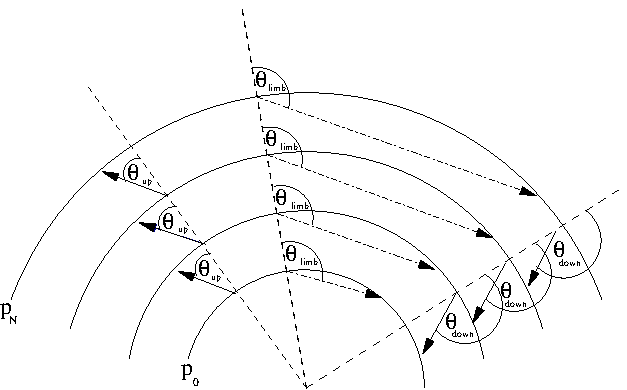
\includegraphics[width=.8\hsize]{seq_update_bw}
 \caption{Schematic of the sequential update (1D) showing the three different parts:  ``up-looking'' corresponds to zenith angles $\ZntAng_\mathrm{up}$, ``limb-looking'' corresponds to $\ZntAng_\mathrm{limb}$ ``down-looking'' corresponds to $\ZntAng_\mathrm{down}$.}
  \label{fig:scattering:seq_update}  
\end{figure}

The \emph{boundary condition} for the calculation is the incoming
radiation field on the cloud box boundary $\IFld^{bd}$:
\begin{eqnarray}
  \IFld^{bd} = \left\{\StoVec \left( \Prs_i,\ZntAng_l \right) \right\}
  \: \mathrm{where}  \: & \Prs_i = \Prs_N \, \forall \,  \ZntAng_l \in [0,\ZntAng_\mathrm{limit}]  \nonumber\\
   & \Prs_i = \Prs_0  \, \forall \, \ZntAng_l \in (\ZntAng_\mathrm{limit},180^\circ],
\end{eqnarray}
where $\Prs_0$ and $\Prs_N$ are the pressure coordinates of the lower and
upper cloud box boundaries respectively. For down-looking directions,
the intensity field at the lower-most cloud box boundary and for up-
and limb-looking directions the intensity field at the uppermost
cloud box boundary are the required boundary conditions respectively.

\subsection{Up-looking directions}

The first step of the sequential update is to calculate the intensity
field for the pressure coordinate $\Prs_{N-1}$, the pressure level below
the uppermost boundary, for all up-looking directions.  Radiative
transfer steps are calculated for paths starting at the uppermost
boundary and propagating to the ($N-1$) pressure level. The required
input for this radiative transfer step are the averaged coefficients
of the uppermost cloud box layer and the Stokes vectors at
the uppermost boundary for all up-looking directions. These are obtained
by interpolating the boundary condition $\IFld^{bd}$ on the
appropriate zenith angles. Note that the zenith angle of the
propagation path for the observing direction $\ZntAng_l$ does not equal
$\ZntAng_l'$ at the intersection point due to the spherical
geometry. If $\ZntAng_l$ is close to $90^\circ$\ this difference is
most significant.
  
To calculate the intensity field for the pressure coordinate
$\Prs_{N-2}$, we repeat the calculation above. We have to calculate a
radiative transfer step from the ($N-1$) to the ($N-2$) pressure level.
As input we need the interpolated intensity field at the ($N-1$)
pressure level, which has been calculated in the last step.
  
For each pressure level ($m-1$) we take the interpolated field of the
layer above ($\IFld(\Prs_{m})^{(1)}$).  Using this method, the
scattering influence from particles in the upper-most cloud box
layer can propagate during one iteration down to the lower-most layer.
This means that the number of iterations does not scale with the
number of pressure levels, which would be the case without sequential
update.
  
The radiation field at a specific point in the cloud box is obtained by
solving Equation \ref{eq:scattering:VRTE_sol}. For up-looking directions at position
$\Prs_{m-1}$ we may write:
\begin{eqnarray}
 & \StoVec\left( \Prs_{m-1},\ZntAng_\mathrm{up} \right) ^{(1)}  =  
  e^{-\overline{\EnsAvr{\ExtMat (\ZntAng_\mathrm{up})}} s} 
  \StoVec\left( \Prs_m,\ZntAng_\mathrm{up} \right)^{(1)}  \nonumber \\ &+
  \left( \IdnMtr -  e^{-\overline{\EnsAvr{\ExtMat (\ZntAng_\mathrm{up})}} s}\right) 
  \overline{\EnsAvr{\ExtMat(\ZntAng_\mathrm{up})}}^{\,-1} 
  \left( \overline{\EnsAvr{\AbsVec (\ZntAng_\mathrm{up})}}\,  
    \bar{B} +
    \overline{\EnsAvr{\SVec\left(\ZntAng_\mathrm{up} \right)^{(0)}} }
  \right).
\end{eqnarray}
For simplification we write
\begin{equation}
  \StoVec ( \Prs_{m-1},\ZntAng_\mathrm{up})^{(1)} = 
  \MtrStl{A}(\ZntAng_\mathrm{up})  \StoVec\left( \Prs_m,\ZntAng_\mathrm{up} \right)^{(1)} 
  + \MtrStl{B} ( \ZntAng_\mathrm{up}).
\end{equation}
Solving this equation sequentially, starting at the top of the cloud
and finishing at the bottom, we get the updated radiation field for
all up-looking angles.
\begin{equation} \IFld(\Prs_i, \ZntAng_\mathrm{up})^{(1)} =
  \left\{ \StoVec^{(1)} \left( \Prs_i,\ZntAng_l \right) \right\} \qquad
  \forall \; \ZntAng_{l} \in [0, 90^\circ].
\end{equation}

\subsection{Down-looking directions}
The same procedure is done for down-looking directions.  The only
difference is that the starting point is the lower-most pressure level
$\Prs_1$ and the incoming clear sky field at the lower cloud box boundary,
which is interpolated on the required zenith angles, is taken as
boundary condition.  The following equation is solved sequentially,
starting at the bottom of the cloud box and finishing at the top:
\begin{equation}
  \StoVec ( \Prs_{m},\ZntAng_\mathrm{down} ) ^{(1)} = 
  \MtrStl{A}(\ZntAng_\mathrm{down}) \StoVec\left( \Prs_{m-1},\ZntAng_\mathrm{down} \right)^{(1)} 
  + \MtrStl{B}(\ZntAng_\mathrm{down}).
\end{equation}
This yields the updated radiation field for all down-looking angles.
\begin{equation}
  \IFld(\Prs_i, \ZntAng_\mathrm{down})^{(1)} = \left\{ \StoVec^{(1)} \left( \Prs_i,\ZntAng_l \right) \right\}  \qquad
  \forall \;  \ZntAng_l \in [\ZntAng_\mathrm{limit}, 180^\circ].
\end{equation}

\subsection{Limb directions}
A special case for limb directions, which correspond to angles
slightly above 90$^\circ$\, had to be implemented.  If the tangent
point is part of the propagation path step, the intersection point is
exactly at the same pressure level as the starting point.  In this
case the linearly interpolated clear sky field is taken as input for
the radiative transfer calculation, because we do not have an already
updated field for this pressure level:
\begin{equation}
  \StoVec ( \Prs_{m},\ZntAng_\mathrm{limb} ) ^{(1)} =   
  \MtrStl{A}(\ZntAng_\mathrm{limb}) \StoVec\left( \Prs_{m},\ZntAng_\mathrm{limb} \right)^{(0)} 
  + \MtrStl{B}(\ZntAng_\mathrm{limb})
\end{equation}
By solving this equation the missing part of the updated radiation
field is obtained
\begin{equation}
  \IFld(\Prs_i, \ZntAng_\mathrm{limb})^{(1)} = \left\{\StoVec \left( \Prs_i,\ZntAng_l \right) \right\}  \qquad
  \forall \;  \ZntAng_l \in  ]90^\circ, \ZntAng_\mathrm{limit}[
\end{equation}
For all iterations the sequential update is applied. Using this method
the number of iterations depends only on the optical thickness of the
cloud or on the number of multiple-scattering events, not on the
number of pressure levels.


\section{Numerical Issues}
\label{sec:doit:implementation_DOIT}


\subsection{Grid optimization and interpolation}
\label{sec:doit:grid_opt_interp}

The accuracy of the DOIT method depends very much on the
discretization of the zenith angle. The reason is that the intensity
field strongly increases at about $\ZntAng=90^\circ$. For angles
below 90$^\circ$ (``up-looking'' directions) the intensity is very
small compared to angles above 90$^\circ$ (``down-looking''
directions), because the thermal emission from the lower atmosphere
and from the ground is much larger than thermal emission from trace
gases in the upper atmosphere. Figure \ref{fig:scattering:i_field} shows an
example intensity field as a function of zenith angle for different
pressure levels inside a cloud box, which is placed from 7.3 to 12.7\,km
altitude, corresponding to pressure limits of 411\,hPa and 188\,hPa
respectively. The cloud box includes 27 pressure levels. The frequency
of the sample calculation was 318\,GHz. A midlatitude-summer scenario
including water vapor, ozone, nitrogen and oxygen was used.
The atmospheric data was taken from the FASCOD \citep{anderson:86}
and the spectroscopic data was obtained from the HITRAN database
\citep{rothman:98}. For simplicity 
this 1D set-up was chosen for all sample calculations in this section.  As the
intensity (or the Stokes vector) at the intersection point of a
propagation path is obtained by interpolation, large interpolation
errors can occur for zenith angles of about 90$^\circ$ if the zenith
angle grid discretization is too coarse.  Taking a very fine
equidistant zenith angle grid leads to very long computation times.
Therefore a zenith angle grid optimization method is required.

For the computation of the scattering integral it is possible to take
a much coarser zenith angle resolution without losing accuracy.  It
does not make sense to use the zenith angle grid, which is optimized
to represent the radiation field with a certain accuracy. The
integrand is the product of the phase matrix and the radiation field.
The peaks of the phase matrices can be at any zenith angle, depending
on the incoming and the scattered directions. The multiplication
smooths out both the radiation field increase at 90$^\circ$ and the
peaks of the phase matrices.  Test calculations have shown that an
increment of 10$^\circ$ is sufficient. Taking the equidistant grid
saves the computation time of the scattering integral to a very large
extent, because much less grid points are required.

\begin{figure}[htbp]
\centering
  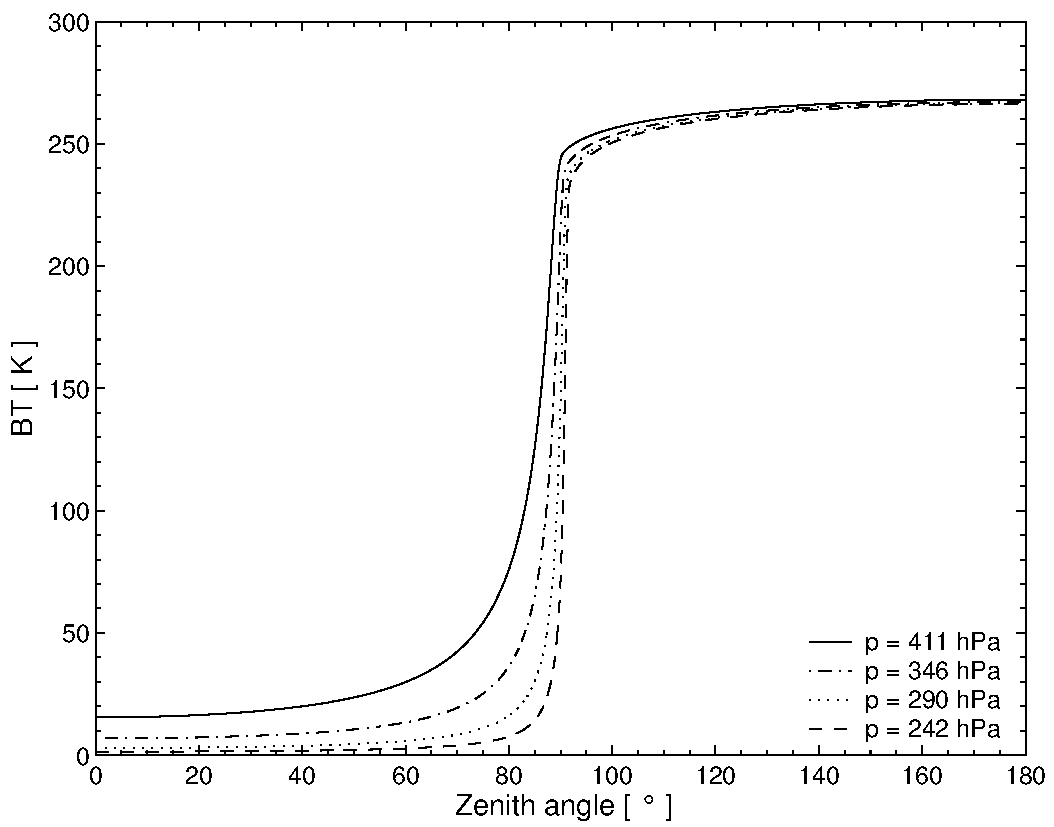
\includegraphics[width=0.8\hsize]{i_field}
  \caption{Intensity field for different pressure levels.}
  \label{fig:scattering:i_field}  
\end{figure}


\subsection{Zenith angle grid optimization}

As a reference field for the grid optimization the DOIT method is
applied for an empty cloud box using a very fine zenith angle grid. The
grid optimization routine finds a reduced zenith angle grid which can
represent the intensity field with the desired accuracy.  It first
takes the radiation at 0$^\circ$ and 180$^\circ$ and interpolates
between these two points on all grid points contained in the fine
zenith angle grid for all pressure levels. Then the differences
between the reference radiation field and the interpolated field are
calculated. The zenith angle grid point, where the difference is
maximal is added to 0$^\circ$ and 180$^\circ$. After that the
radiation field is interpolated between these three points forming 
part of the reduced grid and again the grid point with the maximum
difference is added. Using this method more and more grid points are
added to the reduced grid until the maximum difference is below a
requested accuracy limit.

The top panel of Figure \ref{fig:scattering:grid_acc} shows the clear sky
radiation in all viewing directions for a sensor located at 13\,km
altitude. This result was obtained with a switched-off cloud box.  The
difference between the clear sky part of the ARTS model and the
scattering part is that in the clear sky part the radiative transfer
calculations are done along the line of sight of the instrument
whereas inside the cloud box the RT calculations are done as described
in the previous section to obtain the full radiation field inside the
cloud box. In the clear sky part the radiation field is not
interpolated, therefore we can take the clear sky solution as the exact
solution.

\begin{figure}[t]
\centering
  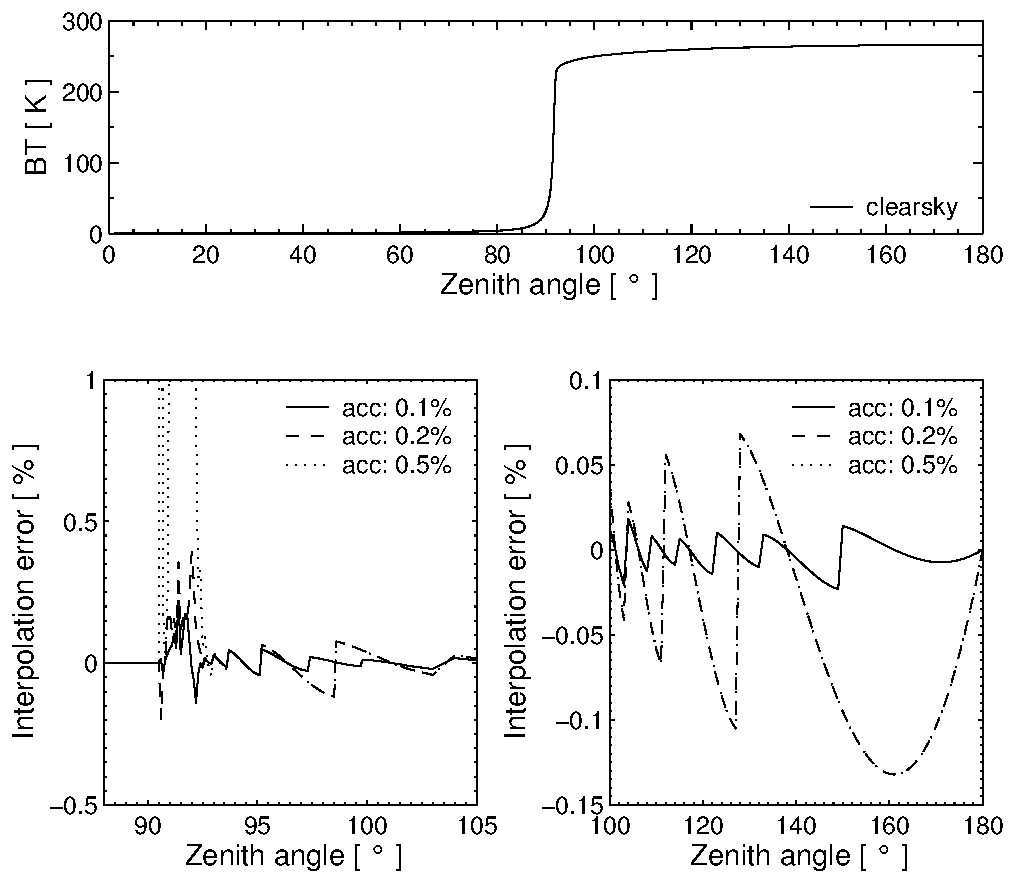
\includegraphics[width=.9\hsize]{grid_acc}
  \caption{Interpolation errors for different grid accuracies.
    Top panel: Clear sky radiation simulated for a sensor at an altitude of
    13\,km for all viewing directions.
    Bottom left: Grid optimization accuracy for limb directions.
    Bottom right: Grid optimization accuracy for down-looking
    directions.}
  \label{fig:scattering:grid_acc}  
\end{figure}

The interpolation error is the relative difference between the exact
clear sky calculation (cloud box switched off) and the clear sky
calculation with empty cloud box.  The bottom panels of
Figure \ref{fig:scattering:grid_acc} show the interpolation errors for zenith
angle grids optimized with three different accuracy limits (0.1\%,
0.2\% and 0.5\%.). The left plot shows the critical region close to
90$^\circ$.  For a grid optimization accuracy of 0.5\% the
interpolation error becomes very large, the maximum error is 
about 8\%. For grid accuracies of 0.2\% and 0.1\% the maximum
interpolation errors are about 0.4\% and 0.2\% respectively. However
for most angles it is below 0.2\%, for all three cases. For
down-looking directions from 100$^\circ$ to 180$^\circ$ the
interpolation error is at most 0.14\% for grid accuracies of 0.2\% and 0.5\%
and for a grid accuracy of 0.1\% it is below~0.02\%. 


\subsection{Interpolation methods}
Two different interpolation methods can be chosen in ARTS for the
interpolation of the radiation field in the zenith angle dimension:
linear interpolation or three-point polynomial interpolation. The polynomial interpolation
method produces more accurate results provided that the zenith angle
grid is optimized appropriately. The linear interpolation method on
the other hand is safer. If the zenith angle grid is not optimized for
polynomial interpolation one should use the simpler linear interpolation
method.  Apart from the interpolation of the radiation field in the
zenith angle dimension linear interpolation is used everywhere in the
model.  Figure \ref{fig:scattering:interp} shows the interpolation errors for the
different interpolation methods.  Both calculations are performed on
optimized zenith angle grids, for polynomial interpolation 65 grid points
were required to achieve an accuracy of 0.1\% and for linear
interpolation 101 points were necessary to achieve the same accuracy.
In the region of about 90$^\circ$ the interpolation errors are below
1.2\% for linear interpolation and below 0.2\% for polynomial
interpolation. For the other down-looking directions the differences
are below 0.08\% for linear and below 0.02\% for polynomial interpolation.
It is obvious that polynomial interpolation gives more accurate results.
Another advantage is that the calculation is faster because less grid
points are required, although the polynomial interpolation method itself is
slower than the linear interpolation method.  Nevertheless, we have
implemented the polynomial interpolation method so far only in the 1D
model. In the 3D model, the grid optimization needs to be done over
the whole cloud box, where it is not obvious that
one can save grid points. Applying the polynomial interpolation method
using non-optimized grids can yield much larger interpolation errors
than the linear interpolation method.

\begin{figure}[htbp]
\centering
  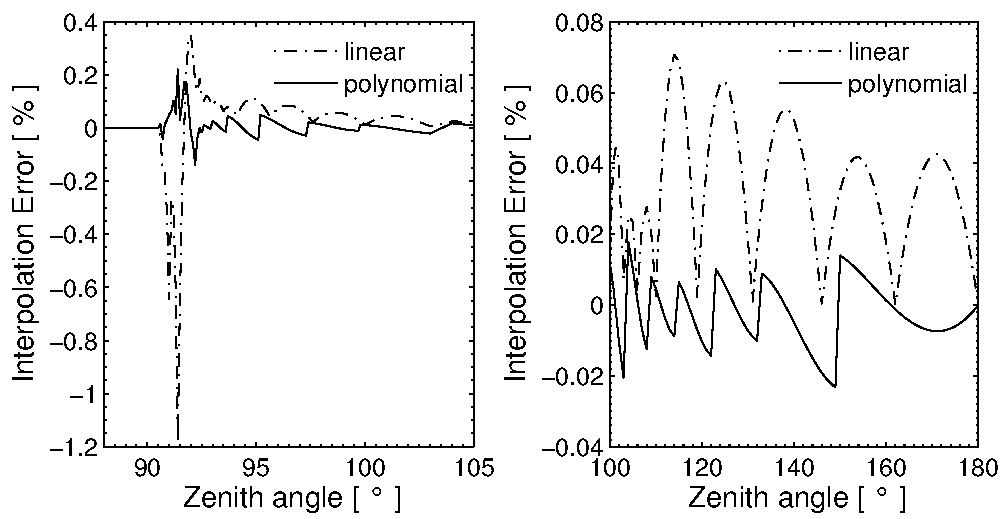
\includegraphics[width=.9\hsize]{interp}
  \caption{Interpolation errors for polynomial and linear interpolation.
  }
  \label{fig:scattering:interp}  
\end{figure}

\subsection{Error estimates}
The interpolation error for scattering calculations can be estimated
by comparison of a scattering calculation performed on a very fine
zenith angle grid (resolution 0.001$^\circ$ from 80$^\circ$ to
100$^\circ$) with a scattering calculation performed on an optimized
zenith angle grid with 0.1\% accuracy. The cloud box used in previous
test calculations is filled with spheroidal particles with an aspect
ratio of 0.5 from 10 to 12\,km altitude. The ice mass content is
assumed to be $4.3\cdot10^{-3}$\,g/m$^3$ at all pressure levels.  
An equal volume sphere radius of 75$\,\mum$ is assumed. The particles are
either completely randomly oriented ("totally\_random") or horizontally aligned
(a special case of "azimuthally\_random" oriented particles) (cf. \user, Section
\ref{U-sec:clouds:particle_types}). The top panels of
Figure \ref{fig:scattering:interp_err} show the interpolation errors of the
intensity.  For both particle orientations the interpolation error is
in the same range as the error for the clear sky calculation, below
0.2\,K. The bottom panels show the interpolation errors for~$Q$. For the
randomly oriented particles the error is below 0.5\%. For the
horizontally aligned particles with random azimuthal orientation it goes up to 2.5\% for a
zenith angle of about 91.5$^\circ$. It is obvious that the
interpolation error for~$Q$ must be larger than that for~$I$ because the
grid optimization is accomplished using only the clear-sky field,
where the polarization is zero. Only the limb directions about
90$^\circ$ are problematic, for other down-looking directions the
interpolation error is below~0.2\%.

\begin{figure}[htbp]
  \centering
  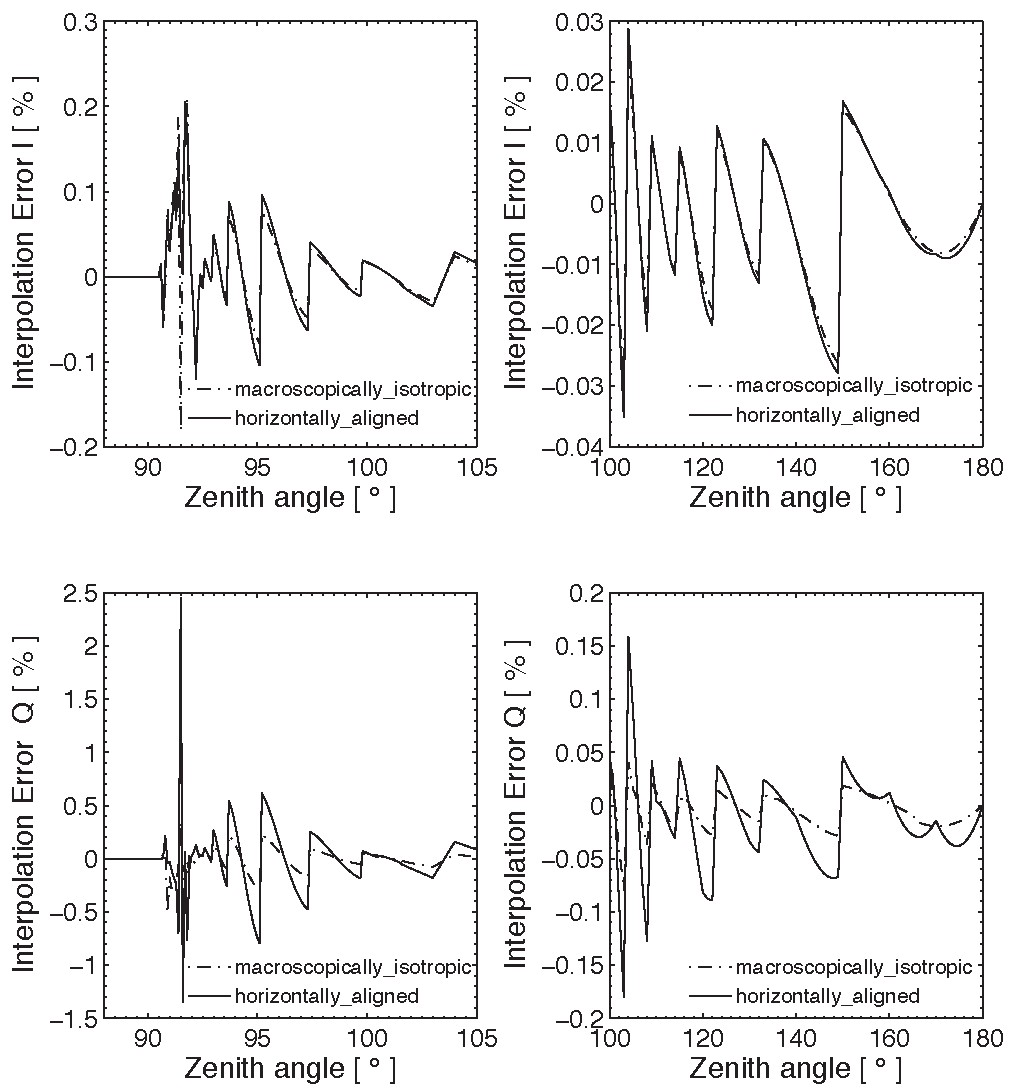
\includegraphics[width=.9\hsize]{interp_err}
  \caption{Interpolation errors for a scattering calculation.
    Left panels: Interpolation errors for limb directions.
    Right panels: Interpolation errors for down-looking directions.
    Top: Intensity~$I$, Bottom: Polarization difference~$Q$}
  \label{fig:scattering:interp_err}  
\end{figure}

